% ===================================================================
%  Week 5 — Edge Detection
% ===================================================================
\documentclass[10pt,aspectratio=169]{beamer}
% ===================================================================
%  Shared Beamer preamble for "Practical Image Processing"
%  English slides. Compile with pdfLaTeX.
% ===================================================================

\usetheme{metropolis}
\usepackage[T1]{fontenc}
\usepackage[utf8]{inputenc}
\usepackage{lmodern}
\usepackage{listings}
\usepackage{tcolorbox}
\usepackage{fontawesome5}
\usepackage{booktabs}
\usepackage{amsmath,amssymb}
\usepackage{tikz}
\usepackage{pgfplots}
\pgfplotsset{compat=1.17}
\usetikzlibrary{arrows.meta,positioning,shapes.geometric,fit,backgrounds,matrix}
\tcbuselibrary{skins,breakable}

% ---- Palette --------------------------------------------------------
\definecolor{coursePrimary}{HTML}{1B4965}   % deep blue
\definecolor{courseAccent}{HTML}{E76F51}    % coral
\definecolor{courseGood}{HTML}{2A9D8F}      % teal
\definecolor{courseBad}{HTML}{C0392B}       % red
\definecolor{courseInfo}{HTML}{2980B9}      % blue
\definecolor{codeBg}{HTML}{F5F6FA}
\definecolor{codeKw}{HTML}{8E44AD}
\definecolor{codeStr}{HTML}{2A9D8F}
\definecolor{codeCom}{HTML}{7F8C8D}

\setbeamercolor{frametitle}{bg=coursePrimary}
\setbeamercolor{progress bar}{fg=courseAccent}
\setbeamercolor{alerted text}{fg=courseAccent}
\metroset{block=fill,sectionpage=progressbar,numbering=fraction}

% ---- Code listings (Python is built into listings) -----------------
\lstdefinestyle{course}{
  backgroundcolor=\color{codeBg},
  basicstyle=\ttfamily\scriptsize,
  keywordstyle=\color{codeKw}\bfseries,
  stringstyle=\color{codeStr},
  commentstyle=\color{codeCom}\itshape,
  numberstyle=\tiny\color{codeCom},
  numbers=left, numbersep=6pt,
  showstringspaces=false, breaklines=true, breakatwhitespace=true,
  tabsize=4, columns=fullflexible,
  frame=single, framesep=4pt, rulecolor=\color{gray!30},
  keepspaces=true, upquote=true, language=Python,
}
\lstset{style=course}
\lstdefinelanguage{bash}{
  keywords={cd,pip,python,venv,source,import}, sensitive=true,
  morecomment=[l]{\#}, morestring=[b]', morestring=[b]",
}

% ---- Reusable callout boxes ----------------------------------------
\newtcolorbox{goodbox}[1][Good practice]{colback=courseGood!8,colframe=courseGood,
  fonttitle=\bfseries,title={\faCheck~#1},boxrule=0.6pt,left=4pt,right=4pt,top=3pt,bottom=3pt}
\newtcolorbox{badbox}[1][Pitfall]{colback=courseBad!8,colframe=courseBad,
  fonttitle=\bfseries,title={\faTimes~#1},boxrule=0.6pt,left=4pt,right=4pt,top=3pt,bottom=3pt}
\newtcolorbox{infobox}[1][Note]{colback=courseInfo!8,colframe=courseInfo,
  fonttitle=\bfseries,title={\faInfoCircle~#1},boxrule=0.6pt,left=4pt,right=4pt,top=3pt,bottom=3pt}
\newtcolorbox{mathbox}[1][Math]{colback=coursePrimary!6,colframe=coursePrimary,
  fonttitle=\bfseries,title={\faCalculator~#1},boxrule=0.6pt,left=4pt,right=4pt,top=3pt,bottom=3pt}

\newcommand{\keyidea}[1]{\begin{alertblock}{Key idea}#1\end{alertblock}}
\newcommand{\term}[1]{\textbf{\color{coursePrimary}#1}}
\newcommand{\code}[1]{\lstinline[basicstyle=\ttfamily\small]|#1|}

% ---- A helper to draw a small pixel grid, cells shaded by value ----
% \pixelgrid{ {10,20,120,200,240}, {30,60,130,180,230}, ... }
\newcommand{\pixelgrid}[1]{%
  \begin{tikzpicture}[font=\scriptsize,scale=0.6]
    \foreach \row [count=\ry] in {#1} {
      \foreach \val [count=\cx] in \row {
        \draw[gray,fill=coursePrimary!8] (\cx,-\ry) rectangle ++(1,-1);
        \node at (\cx+0.5,-\ry-0.5) {\val};
      }
    }
  \end{tikzpicture}}


\title{Edge Detection}
\subtitle{Week 5 — Finding boundaries with gradients}
\author{Practical Image Processing}
\date{Lecture 5 \textbullet\ 60--70 min}

\begin{document}

\maketitle

\begin{frame}{Recap \& today}
  \begin{columns}[T]
    \begin{column}{0.58\textwidth}
      \begin{itemize}
        \item Wk3--4: smoothing/denoising with kernels.
        \item \alert{Today:} \term{edges} — where intensity changes sharply. We find them with
              \term{gradients} (a high-pass kernel), then build up to \term{Canny}.
      \end{itemize}
    \end{column}
    \begin{column}{0.42\textwidth}
      \begin{alertblock}{DocScan milestone}
        Detecting the page/meter boundary starts with edges. This week's output feeds the
        ``find the page'' step.
      \end{alertblock}
    \end{column}
  \end{columns}
\end{frame}

\begin{frame}{Roadmap}\tableofcontents\end{frame}

% ==================================================================
\section{What is an edge?}
% ==================================================================

\begin{frame}{An edge = a rapid intensity change}
  \begin{itemize}
    \item Where the image jumps from dark to light (or vice versa) — object boundaries, text strokes.
    \item Mathematically, a large \term{gradient}: the derivative of intensity is high there.
    \item Edges are \term{high-frequency} (Week 3) — so we detect them with a high-pass kernel.
  \end{itemize}
  \begin{mathbox}
    Gradient magnitude $|\nabla f| = \sqrt{f_x^2 + f_y^2}$; direction $\theta=\operatorname{atan2}(f_y,f_x)$.
  \end{mathbox}
\end{frame}

\begin{frame}{Derivatives as kernels}
  \begin{columns}[T]
    \begin{column}{0.5\textwidth}
      \term{Sobel-x} (vertical edges):
      \[\begin{bmatrix}-1&0&1\\-2&0&2\\-1&0&1\end{bmatrix}\]
    \end{column}
    \begin{column}{0.5\textwidth}
      \term{Sobel-y} (horizontal edges):
      \[\begin{bmatrix}-1&-2&-1\\0&0&0\\1&2&1\end{bmatrix}\]
    \end{column}
  \end{columns}
  \vspace{4pt}
  Each computes a \emph{difference} across the pixel — a discrete derivative. Sum to 0
  (flat regions give 0, as an edge kernel should).
\end{frame}

\begin{frame}{Sobel on the real meter}
  \begin{columns}[T]
    \begin{column}{0.25\textwidth}\begin{center}
      
\includegraphics[width=\linewidth]{../assets/meter_gray.png}\\{\scriptsize gray}
    \end{center}\end{column}
    \begin{column}{0.25\textwidth}\begin{center}
      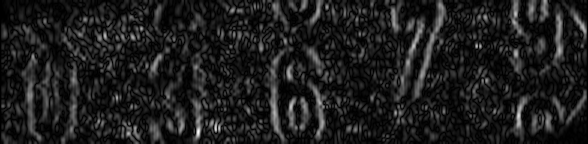
\includegraphics[width=\linewidth]{../assets/meter_sobelx.png}\\{\scriptsize $\partial x$ (vertical edges)}
    \end{center}\end{column}
    \begin{column}{0.25\textwidth}\begin{center}
      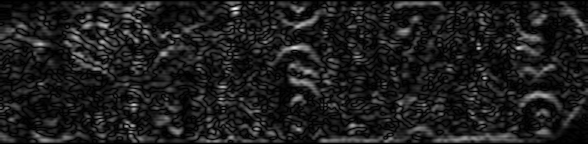
\includegraphics[width=\linewidth]{../assets/meter_sobely.png}\\{\scriptsize $\partial y$ (horizontal)}
    \end{center}\end{column}
    \begin{column}{0.25\textwidth}\begin{center}
      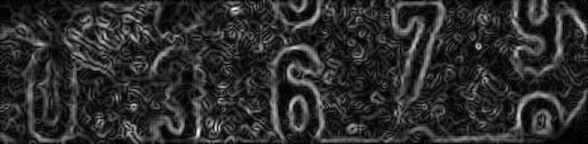
\includegraphics[width=\linewidth]{../assets/meter_sobelmag.png}\\{\scriptsize magnitude}
    \end{center}\end{column}
  \end{columns}
  \vspace{3pt}
  $x$-gradient highlights vertical strokes; $y$-gradient horizontal ones; magnitude combines both.
\end{frame}

\begin{frame}{Gradient magnitude \& direction}
  \begin{itemize}
    \item \term{Magnitude} $= \sqrt{g_x^2 + g_y^2}$: how strong the edge is (the bright edge map).
    \item \term{Direction} $= \operatorname{atan2}(g_y, g_x)$: which way the edge points (used by Canny).
    \item Threshold the magnitude to get a binary edge map — but a fixed threshold is fragile.
  \end{itemize}
  \begin{badbox}
    Gradients are noise-sensitive: noise creates strong fake gradients. Always smooth first (Week 3/4).
  \end{badbox}
\end{frame}

% ==================================================================
\section{Second derivatives}
% ==================================================================

\begin{frame}{Laplacian: the second derivative}
  \begin{columns}[T]
    \begin{column}{0.5\textwidth}
      \[\text{Laplacian }= \begin{bmatrix}0&1&0\\1&-4&1\\0&1&0\end{bmatrix}\]
      Detects edges as \term{zero-crossings} (where the 2nd derivative flips sign).
    \end{column}
    \begin{column}{0.5\textwidth}\begin{center}
      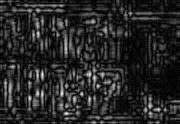
\includegraphics[width=0.9\linewidth]{../assets/plate_laplacian.png}\\{\scriptsize Laplacian of a plate}
    \end{center}\end{column}
  \end{columns}
  \vspace{3pt}
  \begin{itemize}
    \item One kernel finds edges in all directions — but even more noise-sensitive.
    \item \term{LoG} (Laplacian of Gaussian) smooths first, then applies the Laplacian.
  \end{itemize}
\end{frame}

\begin{frame}{The operator family}
  \begin{center}
  \begin{tabular}{@{}lll@{}}
    \toprule
    \textbf{Operator} & \textbf{Idea} & \textbf{Notes} \\
    \midrule
    Roberts & 2$\times$2 diagonal diff & tiny, very noise-sensitive \\
    Prewitt & 3$\times$3, equal weights & simple gradient \\
    Sobel & 3$\times$3, centre-weighted & the practical default \\
    Scharr & optimized 3$\times$3 & better rotational accuracy \\
    Laplacian & 2nd derivative & all directions, one kernel \\
    \bottomrule
  \end{tabular}
  \end{center}
  \keyidea{They all estimate a derivative. Sobel/Scharr are the go-to first-derivative operators.}
\end{frame}

% ==================================================================
\section{The Canny edge detector}
% ==================================================================

\begin{frame}{Canny: the gold-standard pipeline}
  \begin{enumerate}
    \item \term{Smooth} with a Gaussian (kill noise).
    \item \term{Gradient} magnitude \& direction (Sobel).
    \item \term{Non-maximum suppression}: thin thick edges to 1-pixel ridges.
    \item \term{Double threshold + hysteresis}: keep strong edges, and weak ones \emph{connected} to strong.
  \end{enumerate}
  \keyidea{Canny is not a kernel — it's a 4-step algorithm that produces clean, thin, connected edges.}
\end{frame}

\begin{frame}{Canny on real images}
  \begin{columns}[T]
    \begin{column}{0.5\textwidth}\begin{center}
      
\includegraphics[width=0.9\linewidth]{../assets/meter_gray.png}\\{\scriptsize meter}\\[3pt]
      
\includegraphics[width=0.9\linewidth]{../assets/meter_canny.png}\\{\scriptsize Canny edges}
    \end{center}\end{column}
    \begin{column}{0.5\textwidth}\begin{center}
      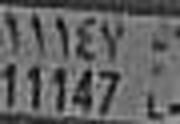
\includegraphics[width=0.7\linewidth]{../assets/plate_gray.png}\\{\scriptsize plate}\\[3pt]
      
\includegraphics[width=0.7\linewidth]{../assets/plate_canny.png}\\{\scriptsize Canny edges}
    \end{center}\end{column}
  \end{columns}
\end{frame}

\begin{frame}{Hysteresis: the clever part}
  \begin{itemize}
    \item Two thresholds: \term{high} (definitely an edge) and \term{low} (maybe).
    \item Keep every strong edge, plus weak edges that \emph{touch} a strong one — drop isolated weak ones.
    \item This bridges gaps along a real edge while rejecting scattered noise responses.
  \end{itemize}
  \begin{goodbox}
    Hysteresis is why Canny gives long, connected contours instead of a speckled mess.
  \end{goodbox}
\end{frame}

\begin{frame}[fragile]{Canny in code + tuning}
\begin{lstlisting}[language=Python]
blur  = cv2.GaussianBlur(gray, (5, 5), 0)     # step 1: smooth
edges = cv2.Canny(blur, 80, 160)              # low=80, high=160
# rule of thumb: high ~= 2-3x low; set from the median intensity (auto-Canny)
\end{lstlisting}
  \begin{badbox}
    Skipping the blur (or thresholds too low) floods the image with noise edges — compare
    \code{Canny(80,160)} to a low-threshold run.
  \end{badbox}
\end{frame}

% ==================================================================
\section{In-class exercise}
% ==================================================================

\begin{frame}{\faPen~In-class exercise (12 min)}
  \begin{infobox}[Reason about a 1D signal]
  \end{infobox}
  A row of pixels: \code{[10, 10, 10, 200, 200, 200]}.
  \begin{enumerate}
    \item Where is the edge? What is the (first) derivative at each gap (differences)?
    \item Where is the derivative \emph{maximum}? Relate that to ``gradient = edge''.
    \item If one pixel were noise (\code{[10,10,90,200,200,200]}), how would a gradient react — and how does smoothing help?
  \end{enumerate}
\end{frame}

\begin{frame}{\faPen~Debrief}
  \begin{itemize}
    \item Differences: \code{[0,0,190,0,0]} — the derivative spikes at the $10\rightarrow200$ jump. That spike \emph{is} the edge.
    \item Max derivative = the edge location. Thresholding the derivative finds edges.
    \item The noise pixel (90) creates a smaller spurious gradient; smoothing averages it away before it becomes a false edge.
  \end{itemize}
  \keyidea{An edge is where the derivative is large. Everything this week is a way to compute and clean that derivative.}
\end{frame}

% ==================================================================
\section{Deep dive}
% ==================================================================

\begin{frame}{Why smooth before differentiating}
  \begin{itemize}
    \item Differentiation \term{amplifies} high frequencies — including noise.
    \item So the derivative of a noisy signal is dominated by noise, not edges.
    \item Smooth first (Gaussian), then differentiate — the basis of Sobel/Canny/LoG.
  \end{itemize}
  \begin{mathbox}
    Handy identity: (blur then differentiate) = convolve with the \emph{derivative of the Gaussian} — one kernel.
  \end{mathbox}
\end{frame}

\begin{frame}{Sub-pixel \& oriented edges (brief)}
  \begin{itemize}
    \item Edge \emph{location} can be refined to sub-pixel accuracy by interpolating the gradient — matters for precise measurement (Week 9).
    \item The gradient \emph{direction} lets you find edges of a specific orientation (e.g. only vertical strokes).
    \item Oriented filters (Gabor) respond to edges/texture at a chosen angle and scale.
  \end{itemize}
\end{frame}

\begin{frame}{Choosing thresholds: auto-Canny}
  \begin{itemize}
    \item Fixed thresholds fail across different lightings. Derive them from the image's median.
    \item \code{low = 0.66*median}, \code{high = 1.33*median} is a robust starting recipe.
    \item Then tune on \emph{hard} images (shadowed, low-contrast meter photos).
  \end{itemize}
\end{frame}

\begin{frame}{Edges $\rightarrow$ the DocScan page finder}
  \begin{itemize}
    \item Canny gives the boundary of the page/meter as connected edges.
    \item Next (Week 9): find \term{contours} from these edges, keep the largest 4-sided one — the page.
    \item Then (Week 11): use its 4 corners for perspective correction. This week is step one.
  \end{itemize}
  \keyidea{Edges aren't the goal — they're the raw material for finding \emph{shapes} (Week 9) and \emph{structure}.}
\end{frame}

\begin{frame}{Gradient magnitude vs Canny — what's the difference?}
  \begin{itemize}
    \item Thresholded Sobel magnitude: thick, broken, noisy edges.
    \item Canny: thin (1-pixel), connected, clean — thanks to NMS + hysteresis.
    \item Use raw gradients for texture/feature strength; use Canny when you need clean \emph{contours}.
  \end{itemize}
  \begin{goodbox}
    For finding the page boundary (a contour), Canny. For measuring edge strength, the gradient magnitude.
  \end{goodbox}
\end{frame}

\begin{frame}{Edges and deep learning}
  \begin{itemize}
    \item A CNN's first layer learns edge/gradient filters \emph{automatically} — often resembling Sobel.
    \item So the features you compute by hand today are what a network discovers on its own (Week 13).
    \item Classical edges remain useful: fast, interpretable, no training data needed.
  \end{itemize}
\end{frame}

% ==================================================================
\section{Wrap-up}
% ==================================================================

\begin{frame}{What you should now be able to do}
  \begin{itemize}
    \item Explain edges as large gradients; compute Sobel-x/y, magnitude, direction.
    \item Use the Laplacian/LoG; understand zero-crossings.
    \item Run and tune the 4-step Canny detector; know why each step exists.
    \item Connect edges to the DocScan page-finding pipeline.
  \end{itemize}
\end{frame}

\begin{frame}{This week's deliverable}
  \begin{alertblock}{Due before Week 6 (see \code{project/})}
    \begin{enumerate}
      \item Compute Sobel-x/y and magnitude on a meter; visualize each.
      \item Run Canny; show the effect of smoothing (with vs without) and of the two thresholds.
      \item Implement auto-Canny from the median; compare to hand-tuned thresholds.
      \item DocScan: get clean edges of the page/meter boundary on 3 real photos.
    \end{enumerate}
  \end{alertblock}
\end{frame}

\begin{frame}[standout]
  An edge is where the derivative is large.\\[4pt]
  \normalsize Smooth, differentiate, thin, connect — that's Canny.
\end{frame}

\end{document}
